\documentclass{standalone}
\usepackage{tikz}
\usetikzlibrary{patterns, positioning}


\begin{document}
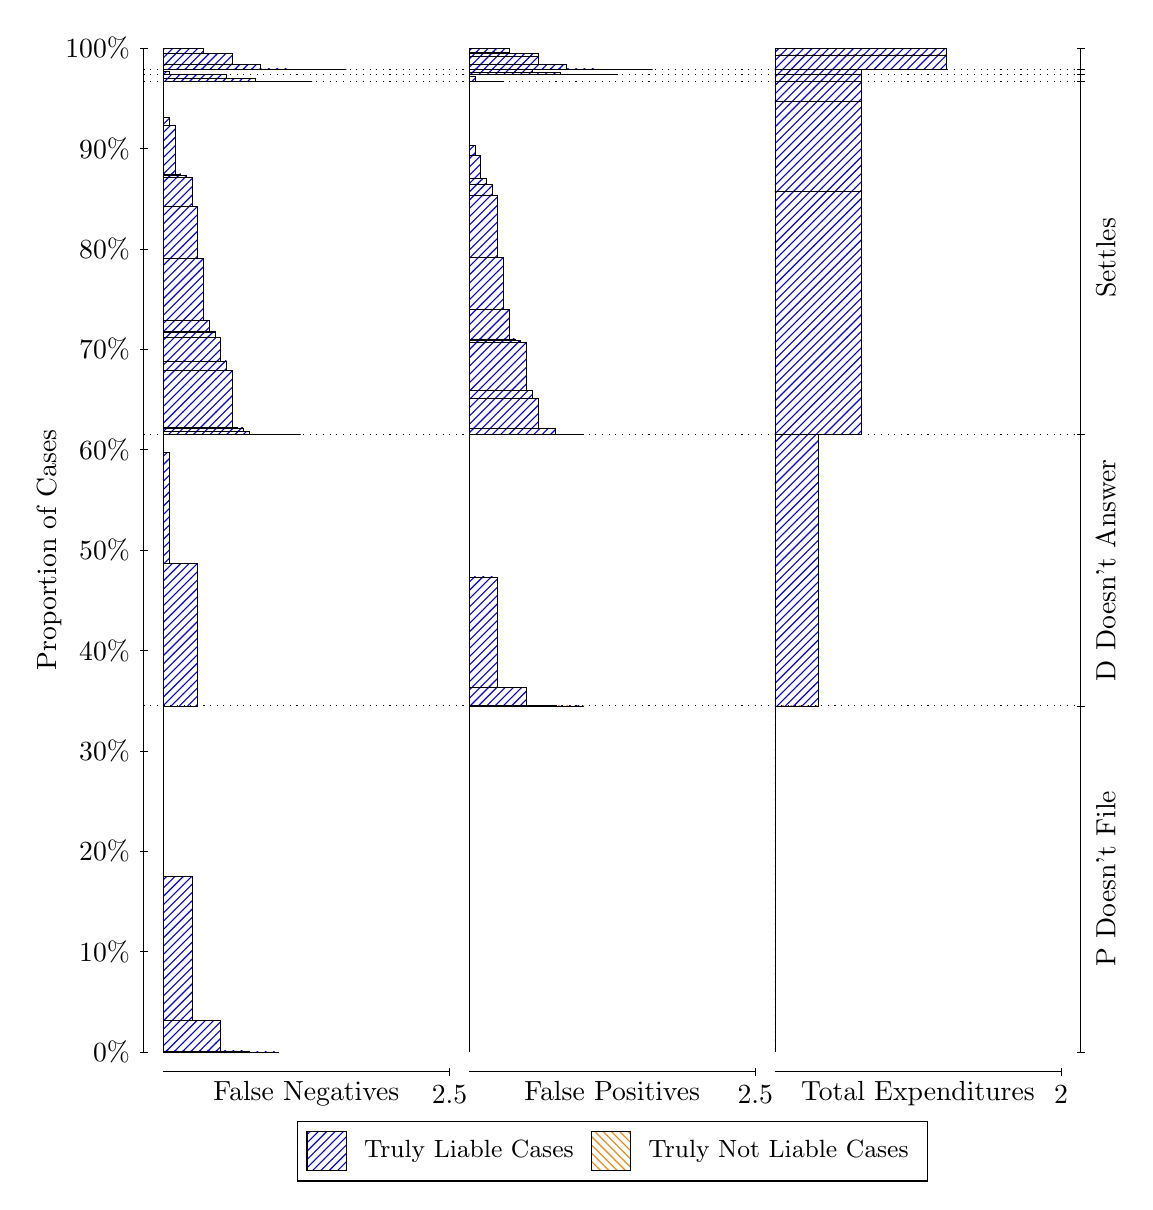
\begin{tikzpicture}
\draw[black, very thin] (1.5,1.75) -- (1.5,14.5);
\node[rotate=90, text=black, anchor=center] at (0.3, 8.125) {Proportion of Cases};
\draw[black, very thin] (1.45,1.75) -- (1.55,1.75);
\node[text=black, anchor=east] at (1.45, 1.75) {0\%};
\draw[black, very thin] (1.45,3.025) -- (1.55,3.025);
\node[text=black, anchor=east] at (1.45, 3.025) {10\%};
\draw[black, very thin] (1.45,4.3) -- (1.55,4.3);
\node[text=black, anchor=east] at (1.45, 4.3) {20\%};
\draw[black, very thin] (1.45,5.575) -- (1.55,5.575);
\node[text=black, anchor=east] at (1.45, 5.575) {30\%};
\draw[black, very thin] (1.45,6.85) -- (1.55,6.85);
\node[text=black, anchor=east] at (1.45, 6.85) {40\%};
\draw[black, very thin] (1.45,8.125) -- (1.55,8.125);
\node[text=black, anchor=east] at (1.45, 8.125) {50\%};
\draw[black, very thin] (1.45,9.4) -- (1.55,9.4);
\node[text=black, anchor=east] at (1.45, 9.4) {60\%};
\draw[black, very thin] (1.45,10.675) -- (1.55,10.675);
\node[text=black, anchor=east] at (1.45, 10.675) {70\%};
\draw[black, very thin] (1.45,11.95) -- (1.55,11.95);
\node[text=black, anchor=east] at (1.45, 11.95) {80\%};
\draw[black, very thin] (1.45,13.225) -- (1.55,13.225);
\node[text=black, anchor=east] at (1.45, 13.225) {90\%};
\draw[black, very thin] (1.45,14.5) -- (1.55,14.5);
\node[text=black, anchor=east] at (1.45, 14.5) {100\%};

\draw[black, very thin] (13.4,1.75) -- (13.4,14.5);
\draw[black, very thin] (13.35,1.75) -- (13.45,1.75);
\node[anchor=west] at (13.35, 1.75) {};
\draw[black, very thin] (13.35,6.1464) -- (13.45,6.1464);
\node[anchor=west] at (13.35, 6.1464) {};
\draw[black, very thin] (13.35,9.5927) -- (13.45,9.5927);
\node[anchor=west] at (13.35, 9.5927) {};
\draw[black, very thin] (13.35,14.078) -- (13.45,14.078);
\node[anchor=west] at (13.35, 14.078) {};
\draw[black, very thin] (13.35,14.169) -- (13.45,14.169);
\node[anchor=west] at (13.35, 14.169) {};
\draw[black, very thin] (13.35,14.23) -- (13.45,14.23);
\node[anchor=west] at (13.35, 14.23) {};
\draw[black, very thin] (13.35,14.5) -- (13.45,14.5);
\node[anchor=west] at (13.35, 14.5) {};

\draw[black, very thin, pattern color=blue, pattern=north east lines] (1.75,1.75) rectangle (3.2033,1.7501);
\draw[black, very thin, pattern color=blue, pattern=north east lines] (1.75,1.7501) rectangle (2.84,1.7628);
\draw[black, very thin, pattern color=blue, pattern=north east lines] (1.75,1.7628) rectangle (2.4767,2.1493);
\draw[black, very thin, pattern color=blue, pattern=north east lines] (1.75,2.1493) rectangle (2.1133,3.9823);
\draw[black, very thin, pattern color=orange, pattern=north west lines] (1.75,3.9823) rectangle (1.75,3.9823);
\draw[black, very thin, pattern color=blue, pattern=north east lines] (1.75,3.9823) rectangle (1.75,6.1464);
\draw[black, very thin, pattern color=blue, pattern=north east lines] (1.75,6.1464) rectangle (2.186,7.9566);
\draw[black, very thin, pattern color=blue, pattern=north east lines] (1.75,7.9566) rectangle (1.8227,9.3606);
\draw[black, very thin, pattern color=orange, pattern=north west lines] (1.75,9.3606) rectangle (1.75,9.3606);
\draw[black, very thin, pattern color=blue, pattern=north east lines] (1.75,9.3606) rectangle (1.75,9.5927);
\draw[black, very thin, pattern color=blue, pattern=north east lines] (1.75,9.5927) rectangle (3.494,9.5927);
\draw[black, very thin, pattern color=blue, pattern=north east lines] (1.75,9.5927) rectangle (3.2033,9.5928);
\draw[black, very thin, pattern color=blue, pattern=north east lines] (1.75,9.5928) rectangle (3.1307,9.5939);
\draw[black, very thin, pattern color=blue, pattern=north east lines] (1.75,9.5939) rectangle (3.058,9.5939);
\draw[black, very thin, pattern color=blue, pattern=north east lines] (1.75,9.5939) rectangle (2.9127,9.5944);
\draw[black, very thin, pattern color=blue, pattern=north east lines] (1.75,9.5944) rectangle (2.84,9.6313);
\draw[black, very thin, pattern color=blue, pattern=north east lines] (1.75,9.6313) rectangle (2.7673,9.6756);
\draw[black, very thin, pattern color=blue, pattern=north east lines] (1.75,9.6756) rectangle (2.6947,9.682);
\draw[black, very thin, pattern color=blue, pattern=north east lines] (1.75,9.682) rectangle (2.622,10.403);
\draw[black, very thin, pattern color=blue, pattern=north east lines] (1.75,10.403) rectangle (2.5493,10.527);
\draw[black, very thin, pattern color=blue, pattern=north east lines] (1.75,10.527) rectangle (2.4767,10.829);
\draw[black, very thin, pattern color=blue, pattern=north east lines] (1.75,10.829) rectangle (2.404,10.894);
\draw[black, very thin, pattern color=blue, pattern=north east lines] (1.75,10.894) rectangle (2.404,10.904);
\draw[black, very thin, pattern color=blue, pattern=north east lines] (1.75,10.904) rectangle (2.3313,11.037);
\draw[black, very thin, pattern color=blue, pattern=north east lines] (1.75,11.037) rectangle (2.2587,11.828);
\draw[black, very thin, pattern color=blue, pattern=north east lines] (1.75,11.828) rectangle (2.186,12.488);
\draw[black, very thin, pattern color=blue, pattern=north east lines] (1.75,12.488) rectangle (2.1133,12.863);
\draw[black, very thin, pattern color=blue, pattern=north east lines] (1.75,12.863) rectangle (2.0407,12.879);
\draw[black, very thin, pattern color=blue, pattern=north east lines] (1.75,12.879) rectangle (2.0407,12.879);
\draw[black, very thin, pattern color=blue, pattern=north east lines] (1.75,12.879) rectangle (1.968,12.902);
\draw[black, very thin, pattern color=blue, pattern=north east lines] (1.75,12.902) rectangle (1.8953,13.515);
\draw[black, very thin, pattern color=blue, pattern=north east lines] (1.75,13.515) rectangle (1.8227,13.621);
\draw[black, very thin, pattern color=orange, pattern=north west lines] (1.75,13.621) rectangle (1.75,13.621);
\draw[black, very thin, pattern color=blue, pattern=north east lines] (1.75,13.621) rectangle (1.75,14.078);
\draw[black, very thin, pattern color=blue, pattern=north east lines] (1.75,14.078) rectangle (3.6393,14.078);
\draw[black, very thin, pattern color=blue, pattern=north east lines] (1.75,14.078) rectangle (3.276,14.078);
\draw[black, very thin, pattern color=blue, pattern=north east lines] (1.75,14.078) rectangle (2.9127,14.112);
\draw[black, very thin, pattern color=blue, pattern=north east lines] (1.75,14.112) rectangle (2.5493,14.168);
\draw[black, very thin, pattern color=blue, pattern=north east lines] (1.75,14.168) rectangle (2.186,14.169);
\draw[black, very thin, pattern color=orange, pattern=north west lines] (1.75,14.169) rectangle (1.75,14.169);
\draw[black, very thin, pattern color=blue, pattern=north east lines] (1.75,14.169) rectangle (2.186,14.17);
\draw[black, very thin, pattern color=blue, pattern=north east lines] (1.75,14.17) rectangle (1.8227,14.207);
\draw[black, very thin, pattern color=orange, pattern=north west lines] (1.75,14.207) rectangle (1.75,14.207);
\draw[black, very thin, pattern color=blue, pattern=north east lines] (1.75,14.207) rectangle (1.75,14.23);
\draw[black, very thin, pattern color=blue, pattern=north east lines] (1.75,14.23) rectangle (4.0753,14.23);
\draw[black, very thin, pattern color=blue, pattern=north east lines] (1.75,14.23) rectangle (3.712,14.23);
\draw[black, very thin, pattern color=blue, pattern=north east lines] (1.75,14.23) rectangle (3.3487,14.234);
\draw[black, very thin, pattern color=blue, pattern=north east lines] (1.75,14.234) rectangle (2.9853,14.297);
\draw[black, very thin, pattern color=blue, pattern=north east lines] (1.75,14.297) rectangle (2.622,14.433);
\draw[black, very thin, pattern color=blue, pattern=north east lines] (1.75,14.433) rectangle (2.2587,14.495);
\draw[black, very thin, pattern color=blue, pattern=north east lines] (1.75,14.495) rectangle (1.8953,14.5);
\draw[black, very thin, pattern color=orange, pattern=north west lines] (1.75,14.5) rectangle (1.75,14.5);
\draw[black, very thin, pattern color=blue, pattern=north east lines] (1.75,14.5) rectangle (1.75,14.5);
\draw[black, very thin, pattern color=orange, pattern=north west lines] (5.6333,1.75) rectangle (5.6333,1.75);
\draw[black, very thin, pattern color=blue, pattern=north east lines] (5.6333,1.75) rectangle (5.6333,6.1464);
\draw[black, very thin, pattern color=orange, pattern=north west lines] (5.6333,6.1464) rectangle (7.0867,6.1464);
\draw[black, very thin, pattern color=blue, pattern=north east lines] (5.6333,6.1464) rectangle (7.0867,6.1464);
\draw[black, very thin, pattern color=blue, pattern=north east lines] (5.6333,6.1464) rectangle (6.7233,6.1475);
\draw[black, very thin, pattern color=blue, pattern=north east lines] (5.6333,6.1475) rectangle (6.36,6.3785);
\draw[black, very thin, pattern color=blue, pattern=north east lines] (5.6333,6.3785) rectangle (5.9967,7.7824);
\draw[black, very thin, pattern color=blue, pattern=north east lines] (5.6333,7.7824) rectangle (5.6333,9.5927);
\draw[black, very thin, pattern color=orange, pattern=north west lines] (5.6333,9.5927) rectangle (7.0867,9.5927);
\draw[black, very thin, pattern color=blue, pattern=north east lines] (5.6333,9.5927) rectangle (7.0867,9.5929);
\draw[black, very thin, pattern color=orange, pattern=north west lines] (5.6333,9.5929) rectangle (6.9413,9.5929);
\draw[black, very thin, pattern color=blue, pattern=north east lines] (5.6333,9.5929) rectangle (6.9413,9.5929);
\draw[black, very thin, pattern color=orange, pattern=north west lines] (5.6333,9.5929) rectangle (6.796,9.5929);
\draw[black, very thin, pattern color=blue, pattern=north east lines] (5.6333,9.5929) rectangle (6.796,9.5932);
\draw[black, very thin, pattern color=blue, pattern=north east lines] (5.6333,9.5932) rectangle (6.7233,9.6672);
\draw[black, very thin, pattern color=orange, pattern=north west lines] (5.6333,9.6672) rectangle (6.6507,9.6672);
\draw[black, very thin, pattern color=blue, pattern=north east lines] (5.6333,9.6672) rectangle (6.6507,9.6674);
\draw[black, very thin, pattern color=blue, pattern=north east lines] (5.6333,9.6674) rectangle (6.578,9.6675);
\draw[black, very thin, pattern color=orange, pattern=north west lines] (5.6333,9.6675) rectangle (6.5053,9.6675);
\draw[black, very thin, pattern color=blue, pattern=north east lines] (5.6333,9.6675) rectangle (6.5053,10.05);
\draw[black, very thin, pattern color=blue, pattern=north east lines] (5.6333,10.05) rectangle (6.4327,10.156);
\draw[black, very thin, pattern color=blue, pattern=north east lines] (5.6333,10.156) rectangle (6.36,10.768);
\draw[black, very thin, pattern color=blue, pattern=north east lines] (5.6333,10.768) rectangle (6.2873,10.791);
\draw[black, very thin, pattern color=orange, pattern=north west lines] (5.6333,10.791) rectangle (6.2147,10.791);
\draw[black, very thin, pattern color=blue, pattern=north east lines] (5.6333,10.791) rectangle (6.2147,10.791);
\draw[black, very thin, pattern color=blue, pattern=north east lines] (5.6333,10.791) rectangle (6.2147,10.807);
\draw[black, very thin, pattern color=blue, pattern=north east lines] (5.6333,10.807) rectangle (6.142,11.182);
\draw[black, very thin, pattern color=blue, pattern=north east lines] (5.6333,11.182) rectangle (6.0693,11.842);
\draw[black, very thin, pattern color=blue, pattern=north east lines] (5.6333,11.842) rectangle (5.9967,12.634);
\draw[black, very thin, pattern color=blue, pattern=north east lines] (5.6333,12.634) rectangle (5.924,12.766);
\draw[black, very thin, pattern color=blue, pattern=north east lines] (5.6333,12.766) rectangle (5.8513,12.776);
\draw[black, very thin, pattern color=blue, pattern=north east lines] (5.6333,12.776) rectangle (5.8513,12.841);
\draw[black, very thin, pattern color=blue, pattern=north east lines] (5.6333,12.841) rectangle (5.7787,13.143);
\draw[black, very thin, pattern color=blue, pattern=north east lines] (5.6333,13.143) rectangle (5.706,13.267);
\draw[black, very thin, pattern color=blue, pattern=north east lines] (5.6333,13.267) rectangle (5.6333,14.078);
\draw[black, very thin, pattern color=orange, pattern=north west lines] (5.6333,14.078) rectangle (6.0693,14.078);
\draw[black, very thin, pattern color=blue, pattern=north east lines] (5.6333,14.078) rectangle (6.0693,14.079);
\draw[black, very thin, pattern color=blue, pattern=north east lines] (5.6333,14.079) rectangle (5.706,14.135);
\draw[black, very thin, pattern color=blue, pattern=north east lines] (5.6333,14.135) rectangle (5.6333,14.169);
\draw[black, very thin, pattern color=orange, pattern=north west lines] (5.6333,14.169) rectangle (7.5227,14.169);
\draw[black, very thin, pattern color=blue, pattern=north east lines] (5.6333,14.169) rectangle (7.5227,14.169);
\draw[black, very thin, pattern color=blue, pattern=north east lines] (5.6333,14.169) rectangle (7.1593,14.169);
\draw[black, very thin, pattern color=blue, pattern=north east lines] (5.6333,14.169) rectangle (6.796,14.192);
\draw[black, very thin, pattern color=blue, pattern=north east lines] (5.6333,14.192) rectangle (6.4327,14.229);
\draw[black, very thin, pattern color=blue, pattern=north east lines] (5.6333,14.229) rectangle (6.0693,14.23);
\draw[black, very thin, pattern color=orange, pattern=north west lines] (5.6333,14.23) rectangle (7.9587,14.23);
\draw[black, very thin, pattern color=blue, pattern=north east lines] (5.6333,14.23) rectangle (7.9587,14.23);
\draw[black, very thin, pattern color=orange, pattern=north west lines] (5.6333,14.23) rectangle (7.5953,14.23);
\draw[black, very thin, pattern color=blue, pattern=north east lines] (5.6333,14.23) rectangle (7.5953,14.23);
\draw[black, very thin, pattern color=orange, pattern=north west lines] (5.6333,14.23) rectangle (7.232,14.23);
\draw[black, very thin, pattern color=blue, pattern=north east lines] (5.6333,14.23) rectangle (7.232,14.234);
\draw[black, very thin, pattern color=blue, pattern=north east lines] (5.6333,14.234) rectangle (6.8687,14.296);
\draw[black, very thin, pattern color=orange, pattern=north west lines] (5.6333,14.296) rectangle (6.8687,14.296);
\draw[black, very thin, pattern color=blue, pattern=north east lines] (5.6333,14.296) rectangle (6.8687,14.297);
\draw[black, very thin, pattern color=blue, pattern=north east lines] (5.6333,14.297) rectangle (6.5053,14.395);
\draw[black, very thin, pattern color=orange, pattern=north west lines] (5.6333,14.395) rectangle (6.5053,14.395);
\draw[black, very thin, pattern color=blue, pattern=north east lines] (5.6333,14.395) rectangle (6.5053,14.433);
\draw[black, very thin, pattern color=blue, pattern=north east lines] (5.6333,14.433) rectangle (6.142,14.45);
\draw[black, very thin, pattern color=blue, pattern=north east lines] (5.6333,14.45) rectangle (6.142,14.496);
\draw[black, very thin, pattern color=blue, pattern=north east lines] (5.6333,14.496) rectangle (5.7787,14.496);
\draw[black, very thin, pattern color=blue, pattern=north east lines] (5.6333,14.496) rectangle (5.7787,14.5);
\draw[black, very thin, pattern color=blue, pattern=north east lines] (5.6333,14.5) rectangle (5.6333,14.5);
\draw[black, very thin, pattern color=orange, pattern=north west lines] (9.5167,1.75) rectangle (9.5167,1.75);
\draw[black, very thin, pattern color=blue, pattern=north east lines] (9.5167,1.75) rectangle (9.5167,6.1464);
\draw[black, very thin, pattern color=orange, pattern=north west lines] (9.5167,6.1464) rectangle (10.062,6.1464);
\draw[black, very thin, pattern color=blue, pattern=north east lines] (9.5167,6.1464) rectangle (10.062,9.5927);
\draw[black, very thin, pattern color=orange, pattern=north west lines] (9.5167,9.5927) rectangle (10.607,9.5927);
\draw[black, very thin, pattern color=blue, pattern=north east lines] (9.5167,9.5927) rectangle (10.607,12.683);
\draw[black, very thin, pattern color=orange, pattern=north west lines] (9.5167,12.683) rectangle (10.607,12.683);
\draw[black, very thin, pattern color=blue, pattern=north east lines] (9.5167,12.683) rectangle (10.607,13.818);
\draw[black, very thin, pattern color=orange, pattern=north west lines] (9.5167,13.818) rectangle (10.607,13.818);
\draw[black, very thin, pattern color=blue, pattern=north east lines] (9.5167,13.818) rectangle (10.607,14.078);
\draw[black, very thin, pattern color=orange, pattern=north west lines] (9.5167,14.078) rectangle (10.607,14.078);
\draw[black, very thin, pattern color=blue, pattern=north east lines] (9.5167,14.078) rectangle (10.607,14.169);
\draw[black, very thin, pattern color=orange, pattern=north west lines] (9.5167,14.169) rectangle (10.607,14.169);
\draw[black, very thin, pattern color=blue, pattern=north east lines] (9.5167,14.169) rectangle (10.607,14.23);
\draw[black, very thin, pattern color=orange, pattern=north west lines] (9.5167,14.23) rectangle (11.697,14.23);
\draw[black, very thin, pattern color=blue, pattern=north east lines] (9.5167,14.23) rectangle (11.697,14.412);
\draw[black, very thin, pattern color=orange, pattern=north west lines] (9.5167,14.412) rectangle (11.697,14.412);
\draw[black, very thin, pattern color=blue, pattern=north east lines] (9.5167,14.412) rectangle (11.697,14.5);
\draw[black, dotted] (1.5,6.1464) -- (13.4,6.1464);
\draw[black, dotted] (1.5,9.5927) -- (13.4,9.5927);
\draw[black, dotted] (1.5,14.078) -- (13.4,14.078);
\draw[black, dotted] (1.5,14.169) -- (13.4,14.169);
\draw[black, dotted] (1.5,14.23) -- (13.4,14.23);
\draw[black, very thin] (1.75,1.5) -- (5.3833,1.5);
\node[text=black, anchor=north] at (3.5667, 1.5) {False Negatives};
\draw[black, very thin] (5.3833,1.45) -- (5.3833,1.55);
\node[text=black, anchor=north] at (5.3833, 1.45) {2.5};

\draw[black, very thin] (5.6333,1.5) -- (9.2667,1.5);
\node[text=black, anchor=north] at (7.45, 1.5) {False Positives};
\draw[black, very thin] (9.2667,1.45) -- (9.2667,1.55);
\node[text=black, anchor=north] at (9.2667, 1.45) {2.5};

\draw[black, very thin] (9.5167,1.5) -- (13.15,1.5);
\node[text=black, anchor=north] at (11.333, 1.5) {Total Expenditures};
\draw[black, very thin] (13.15,1.45) -- (13.15,1.55);
\node[text=black, anchor=north] at (13.15, 1.45) {2};

\node[text=black, centered, rotate=90] at (13.72, 3.9482) {P Doesn't File};
\node[text=black, centered, rotate=90] at (13.72, 7.8695) {D Doesn't Answer};
\node[text=black, centered, rotate=90] at (13.72, 11.835) {Settles};




\draw (7.449999999999999,1.5) node[draw=none] (baseCoordinate) {};
\begin{scope}[align=center]
        \matrix[scale=0.5, draw=black, below=0.5cm of baseCoordinate, nodes={draw}, column sep=0.1cm]{
            \node[rectangle, draw, minimum width=0.5cm, minimum height=0.5cm, pattern color=blue, pattern=north east lines] {}; &
            \node[draw=none, font=\small, text=black] (B) {Truly Liable Cases}; &
            \node[rectangle, draw, minimum width=0.5cm, minimum height=0.5cm, pattern color=orange, pattern=north west lines] {}; &
            \node[draw=none, font=\small, text=black] (B) {Truly Not Liable Cases}; \\
            };
\end{scope}

\end{tikzpicture}
\end{document}